\section{Problem definition}
Essentially, the digital signature is an identity problem.\newline
The public signature is a cryptosystem $(M, C, K, f, f^{-1})$, where:
\begin{itemize}
    \item $M$ is the set of possible cleartext messages;
    \item $C$ is the set of possible cyphered texts;
    \item $K$ is the set of possible keys;
    \item $f$ is the encyphering function;
    \item $f^{-1}$ is the decyphering function.
\end{itemize}
\subsection{Main concept}
The functioning of the digital signature is the following:
\begin{itemize}
    \item Let's assume that the comunication is between two users, $A$ and $B$.
    \item $A$ computes $f_{B}(m)$, where $m \in M$;
    \item $A$ computes $f_{A}^{-1}(A^{n})$, where $A^{n}$ is $A$'s nickname;
    \item $A$ sends $[f_{B}(m), f_{B}(f_{A}^{-1}(A^{n}))]$;\label{dig_sign_sending}
    \item $B$ verifies that $f_{B}^{-1}(f_{B}(m)) = m$;
    \item $B$ verifies that $f_{B}^{-1}(f_{B}(f_{A}^{-1}(A^{n}))) = f_{A}^{-1}(A^{n})$.
\end{itemize}
\begin{figure}[h]
    \centering
    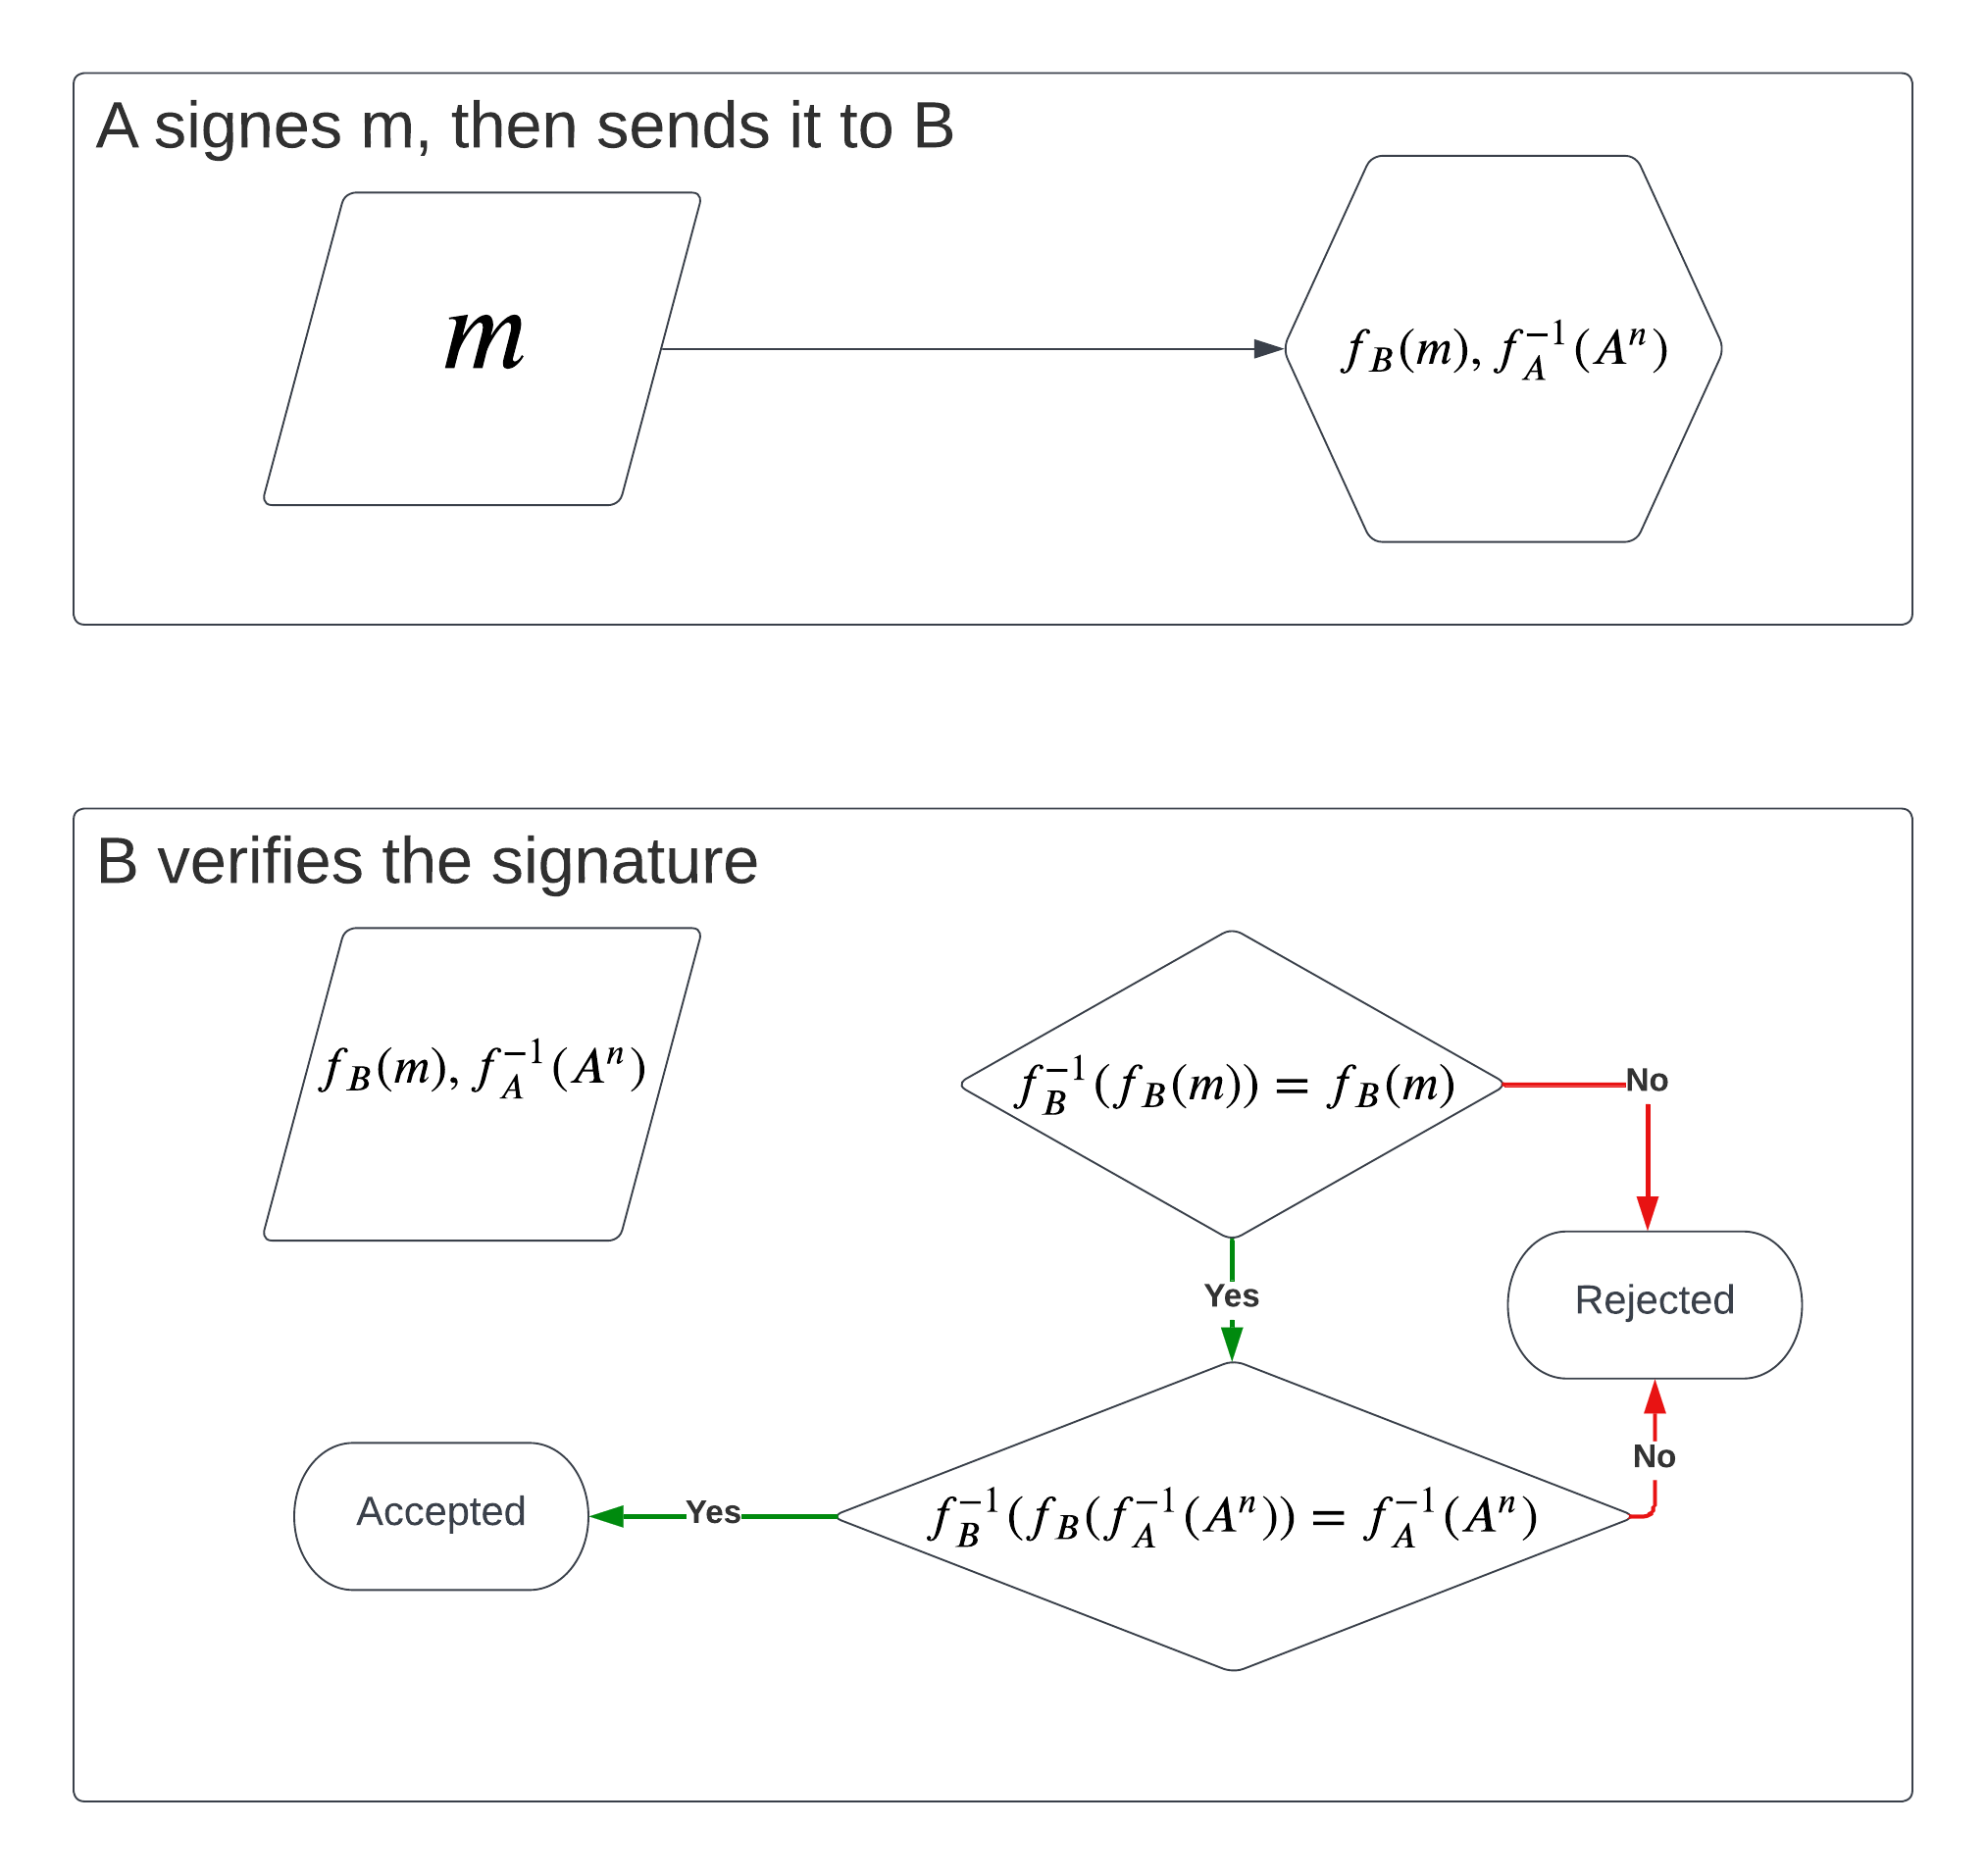
\includegraphics[width=1\textwidth]{img/DigSig.png}
    \caption{Digital Signature in the general case.}
\end{figure}
Since $f_{A}$ is the unique function that can invert $f_{A}^{-1}$, $B$ can verify that the message $m$ is signed from $A$ (actually its nickname). \newline
It's important that $f$ is chosen in such a way that computing $f^{-1}$ is computationally hard without the key. \newline
In this case, \textbf{$f_{A}$ is public} and \textbf{$f_{B}$ is private}.
\subsection{Checking the message's integrity}
An alternative way is to substitute the message at step \ref{dig_sign_sending} with the following:
\[
m_{1}, m_{2} \gets [f_{B}(m), f_{B}(f_{A}^{-1}(m))]
\]
Doing that, $B$ can verify the following identity:
\[
f_{B}^{-1}(f_{B}(m)) = m_{1} \land f_{A}(f_{B}^{-1}(f_{B}(f_{A}^{-1}(m)))) = m_{2}
\]
In this case, \textbf{both $f_{A}$ and $f_{B}$ are public}.

\section{Hash functions}
\begin{definition}[Ideal Hash Function]
    An \textbf{Ideal Hash Function} is a function
    \[
    h: M \rightarrow \{0,1\}^{k}
    \]
    That verifies the following properties:
    \begin{itemize}
        \item \[m \neq m' \implies h(m) \neq h(m')\]
        \item $k \in \mathbb{N}$ and is large enough.
    \end{itemize}
\end{definition}

The goal is to produce $h(m)$ in a such way that a unique input produces a unique output. Since $\operatorname{length}(m)$ is not fixed,this is clearly unfeasible, due to the Pigeonboxes's principles.
Although, it is possible to relax this constraint in the following way:
\begin{definition}[Hash Function]
    An \textbf{Hash Function} is a function
    \[
    h: M \rightarrow \{0,1\}^{k}
    \]
    That verifies the following properties:
    \begin{itemize}
        \item \[\mathbb{P}[h(m) = h(m'): m \neq m'] < 2^{-60}\]
        \item $k \in \mathbb{N}$ and is large enough.
    \end{itemize}
\end{definition}

\subsection{Digital signature with "partial" message integrity check}
An alternative way is to substitute the message at step \ref{dig_sign_sending} with the following:
\[
m_{1}, m_{2} \gets [f_{B}(m), f_{B}(f_{A}^{-1}(h(m)))]
\]
Doing that, $B$ can verify the following identity:
\[
f_{B}^{-1}(f_{B}(m)) = m_{1} \land f_{A}(f_{B}^{-1}(f_{B}(f_{A}^{-1}(h(m))))) = f_{A}(f_{A}^{-1}(h(m)) = h(m)
\]
In this case, \textbf{$f_{A}$ is private} and \textbf{$f_{B}$ is public}. \newline
Since the length of $h(m)$ is fixed, the message is generally smaller, and this can improve the speed of the algorithm.

\subsubsection{Digital signature based on RSA}
This kind of digital signature is based on the following cryptosystem:
\begin{itemize}
    \item For the user $A$: \[M = C = Z_{n_{A}}^{*}\] Where $n_{A} = p_{A} \cdot q_{A}$, and $n_{A}$ is \textbf{public}. Also,
    \[f_{A}(m) = m^{c_{A}} \bmod n_{A}, f_{A}^{-1}(c) = c^{d_{A}} \bmod n_{A}\]
    \item For the user $B$: \[M = C = Z_{n_{B}}^{*}\] Where $n_{B} = p_{B} \cdot q_{B}$, and $n_{B}$ is \textbf{public}. Also,
    \[f_{B}(m) = m^{c_{B}} \bmod n_{B}, f_{B}^{-1}(c) = c^{d_{B}} \bmod n_{B}\]
    \item It's important that $n_{A} \neq n_{B}$.
\end{itemize}
The functioning of this system is the following:
\begin{itemize}
    \item Let $s_{A}$ be the "nickname" of $A$.
    \item $A$ computes $f_{A}^{-1}(f_{B}(s_{A} \bmod n_{B}))$. The module is applied because it can happen that if $n_{A} \geq n_{B}$ the identity could not be verified.
    \item $B$ verifies that
    \[
    f_{B}^{-1}(f_{A}(f_{A}^{-1}(f_{B}(s_{A} \bmod n_{B})))) = s_{A}
    \]
\end{itemize}
\begin{figure}[h]
    \centering
    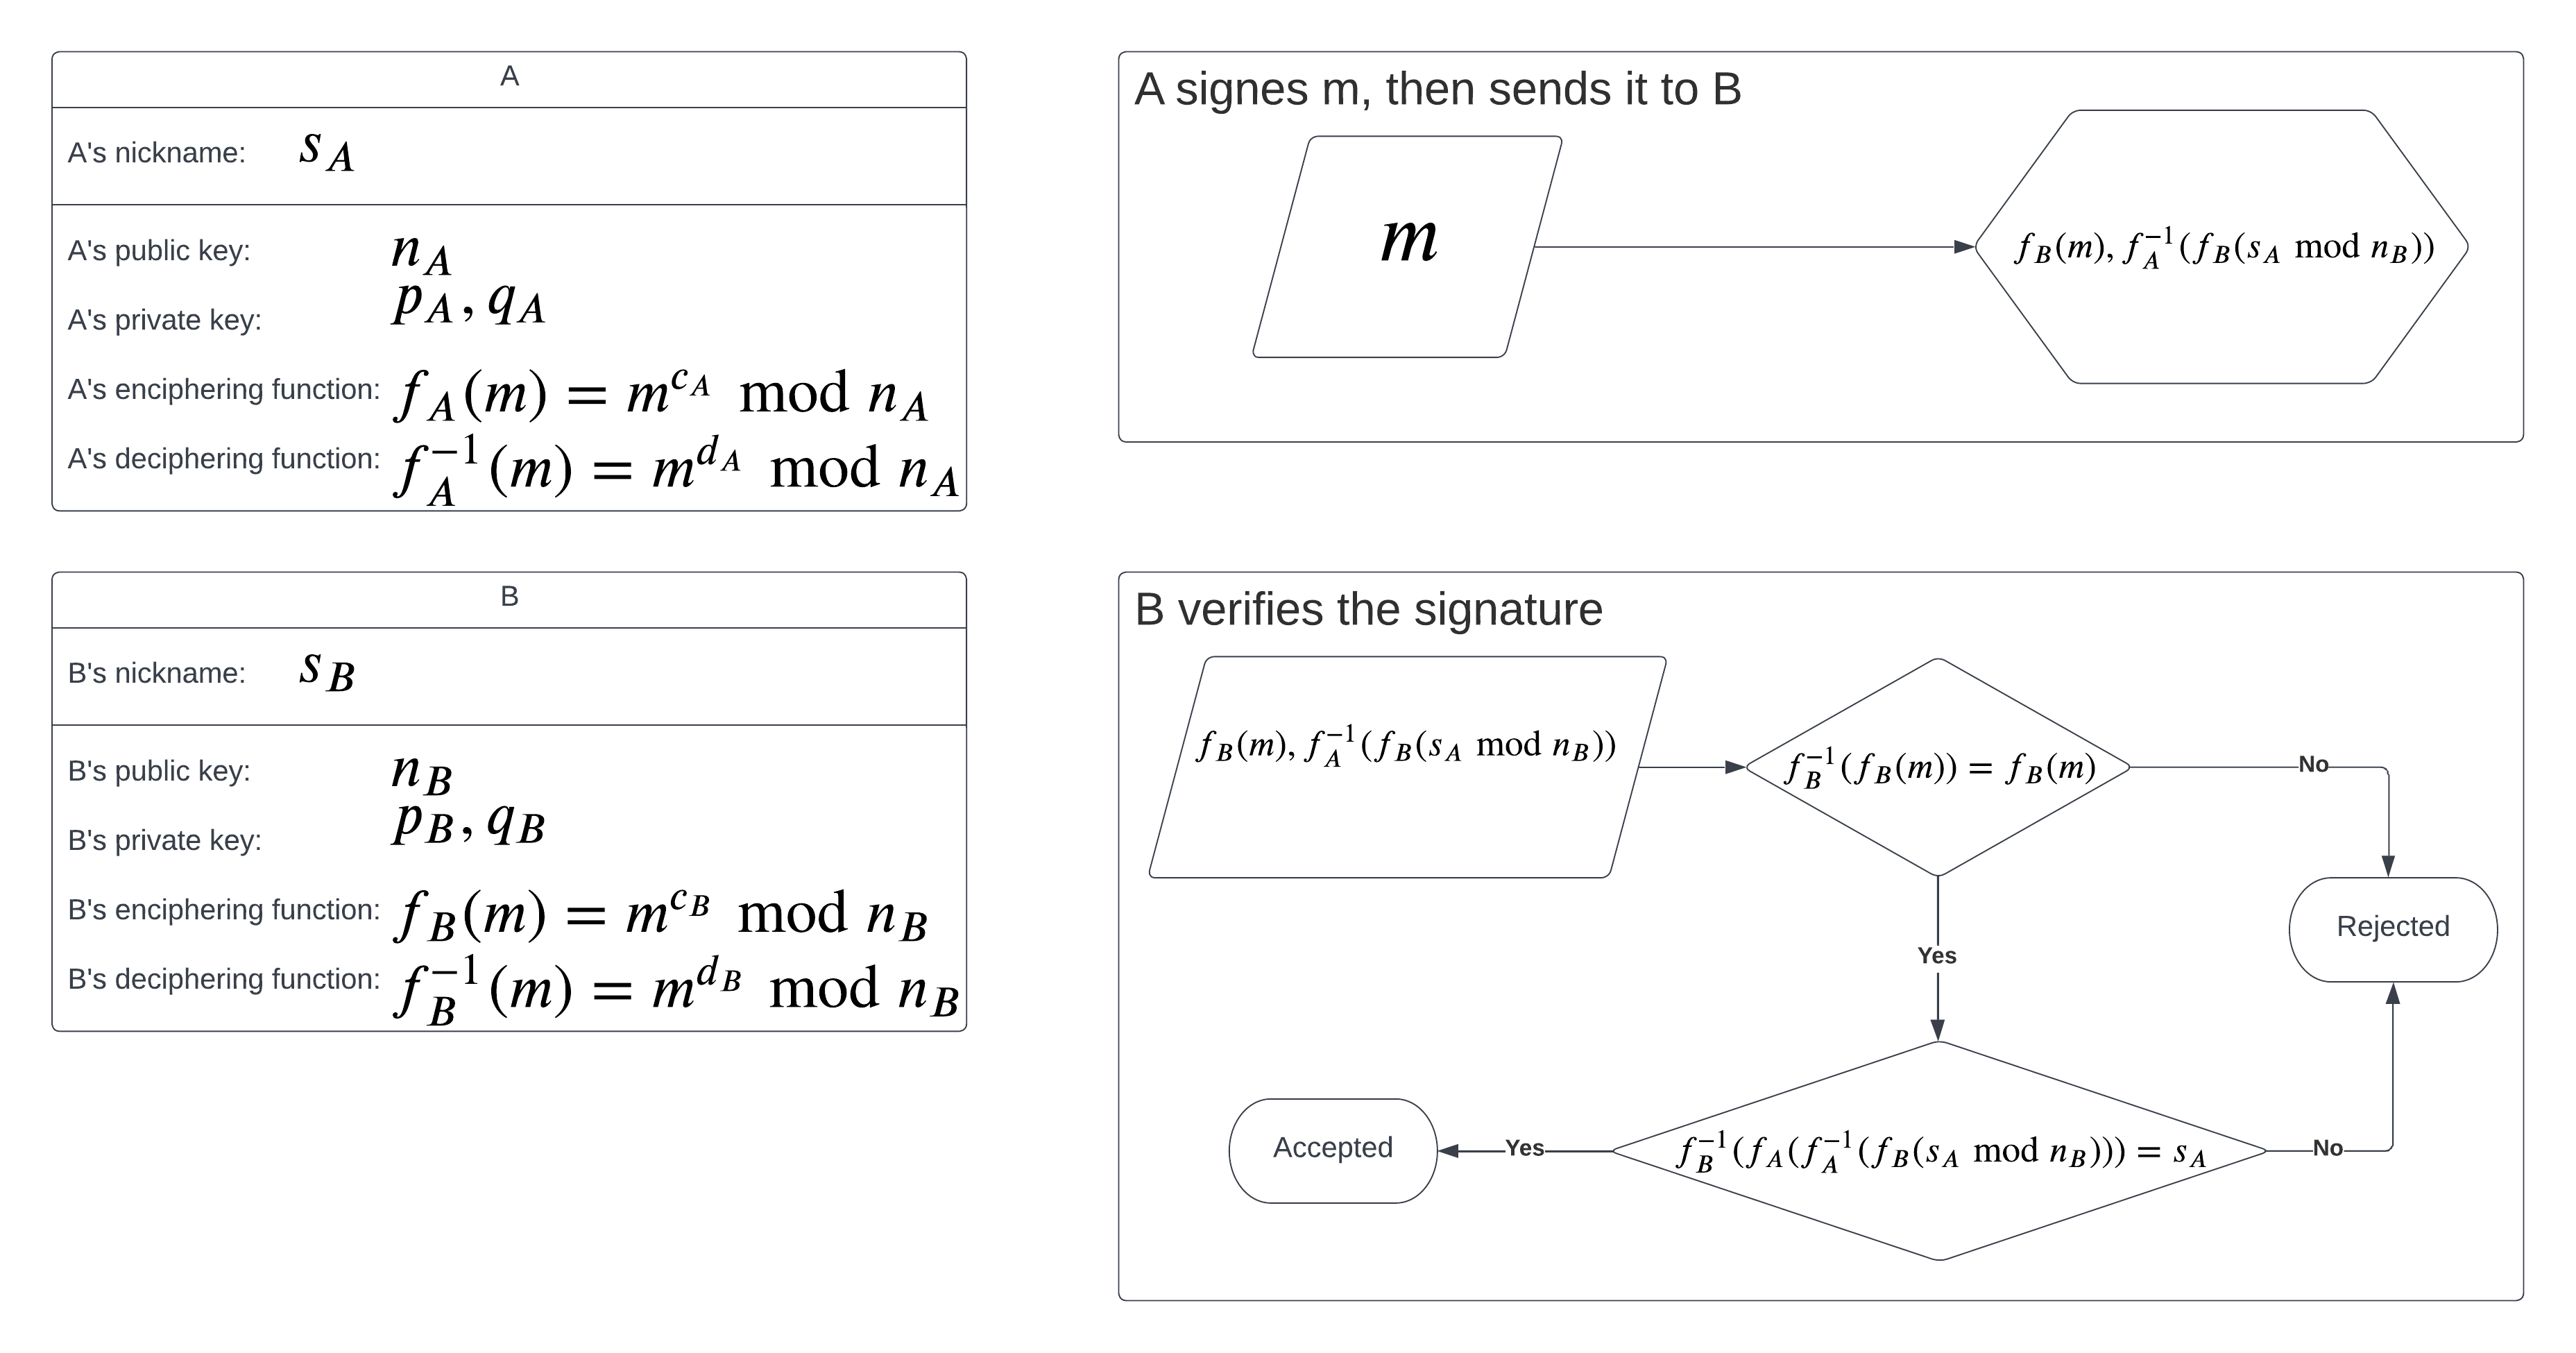
\includegraphics[width=\textwidth]{img/DigSig_RSA.png}
    \caption{Digital signature based on RSA.}
\end{figure}

\subsection{Digital signature based on the ElGamal cryptosystem}
Let's assume that the cryptosystem used is the ElGamal cryptosystem. Let $A, B$ be the users.\newline
In order for $A$ to sign a message $M$:
\begin{enumerate}
    \item $A$ generates $h \in \mathbb{Z}_{p-1}^{*}$. Remark that $h$ is invertible.
    \item $A$ computes $u \equiv_{p} g^{h}$
    \item $A$ computes $v$ such that:
    \begin{align*}
        M &\equiv_{p-1} x \cdot u + h \cdot v\\
        \implies v &\equiv_{p-1} (M - x \cdot u) h^{-1}
    \end{align*}
    Where $x$ is $A$'s private key.
    \item The digital signature is then $(u, v)$.
    \item The message signed appears as $g^{k}, M \cdot b^{k}, (u,v)$
\end{enumerate}

In order for $B$ to verify the signature $g^{k}, M \cdot b^{k}, (u,v)$,
it must compute:
\begin{align*}
    a^{u} \cdot u^{v} &= (g^{x})^{u} \cdot (g^{h})^{v} =\\
    g^{ux + hv} &\equiv g^{M} \bmod p
\end{align*}
\begin{figure}[h]
    \centering
    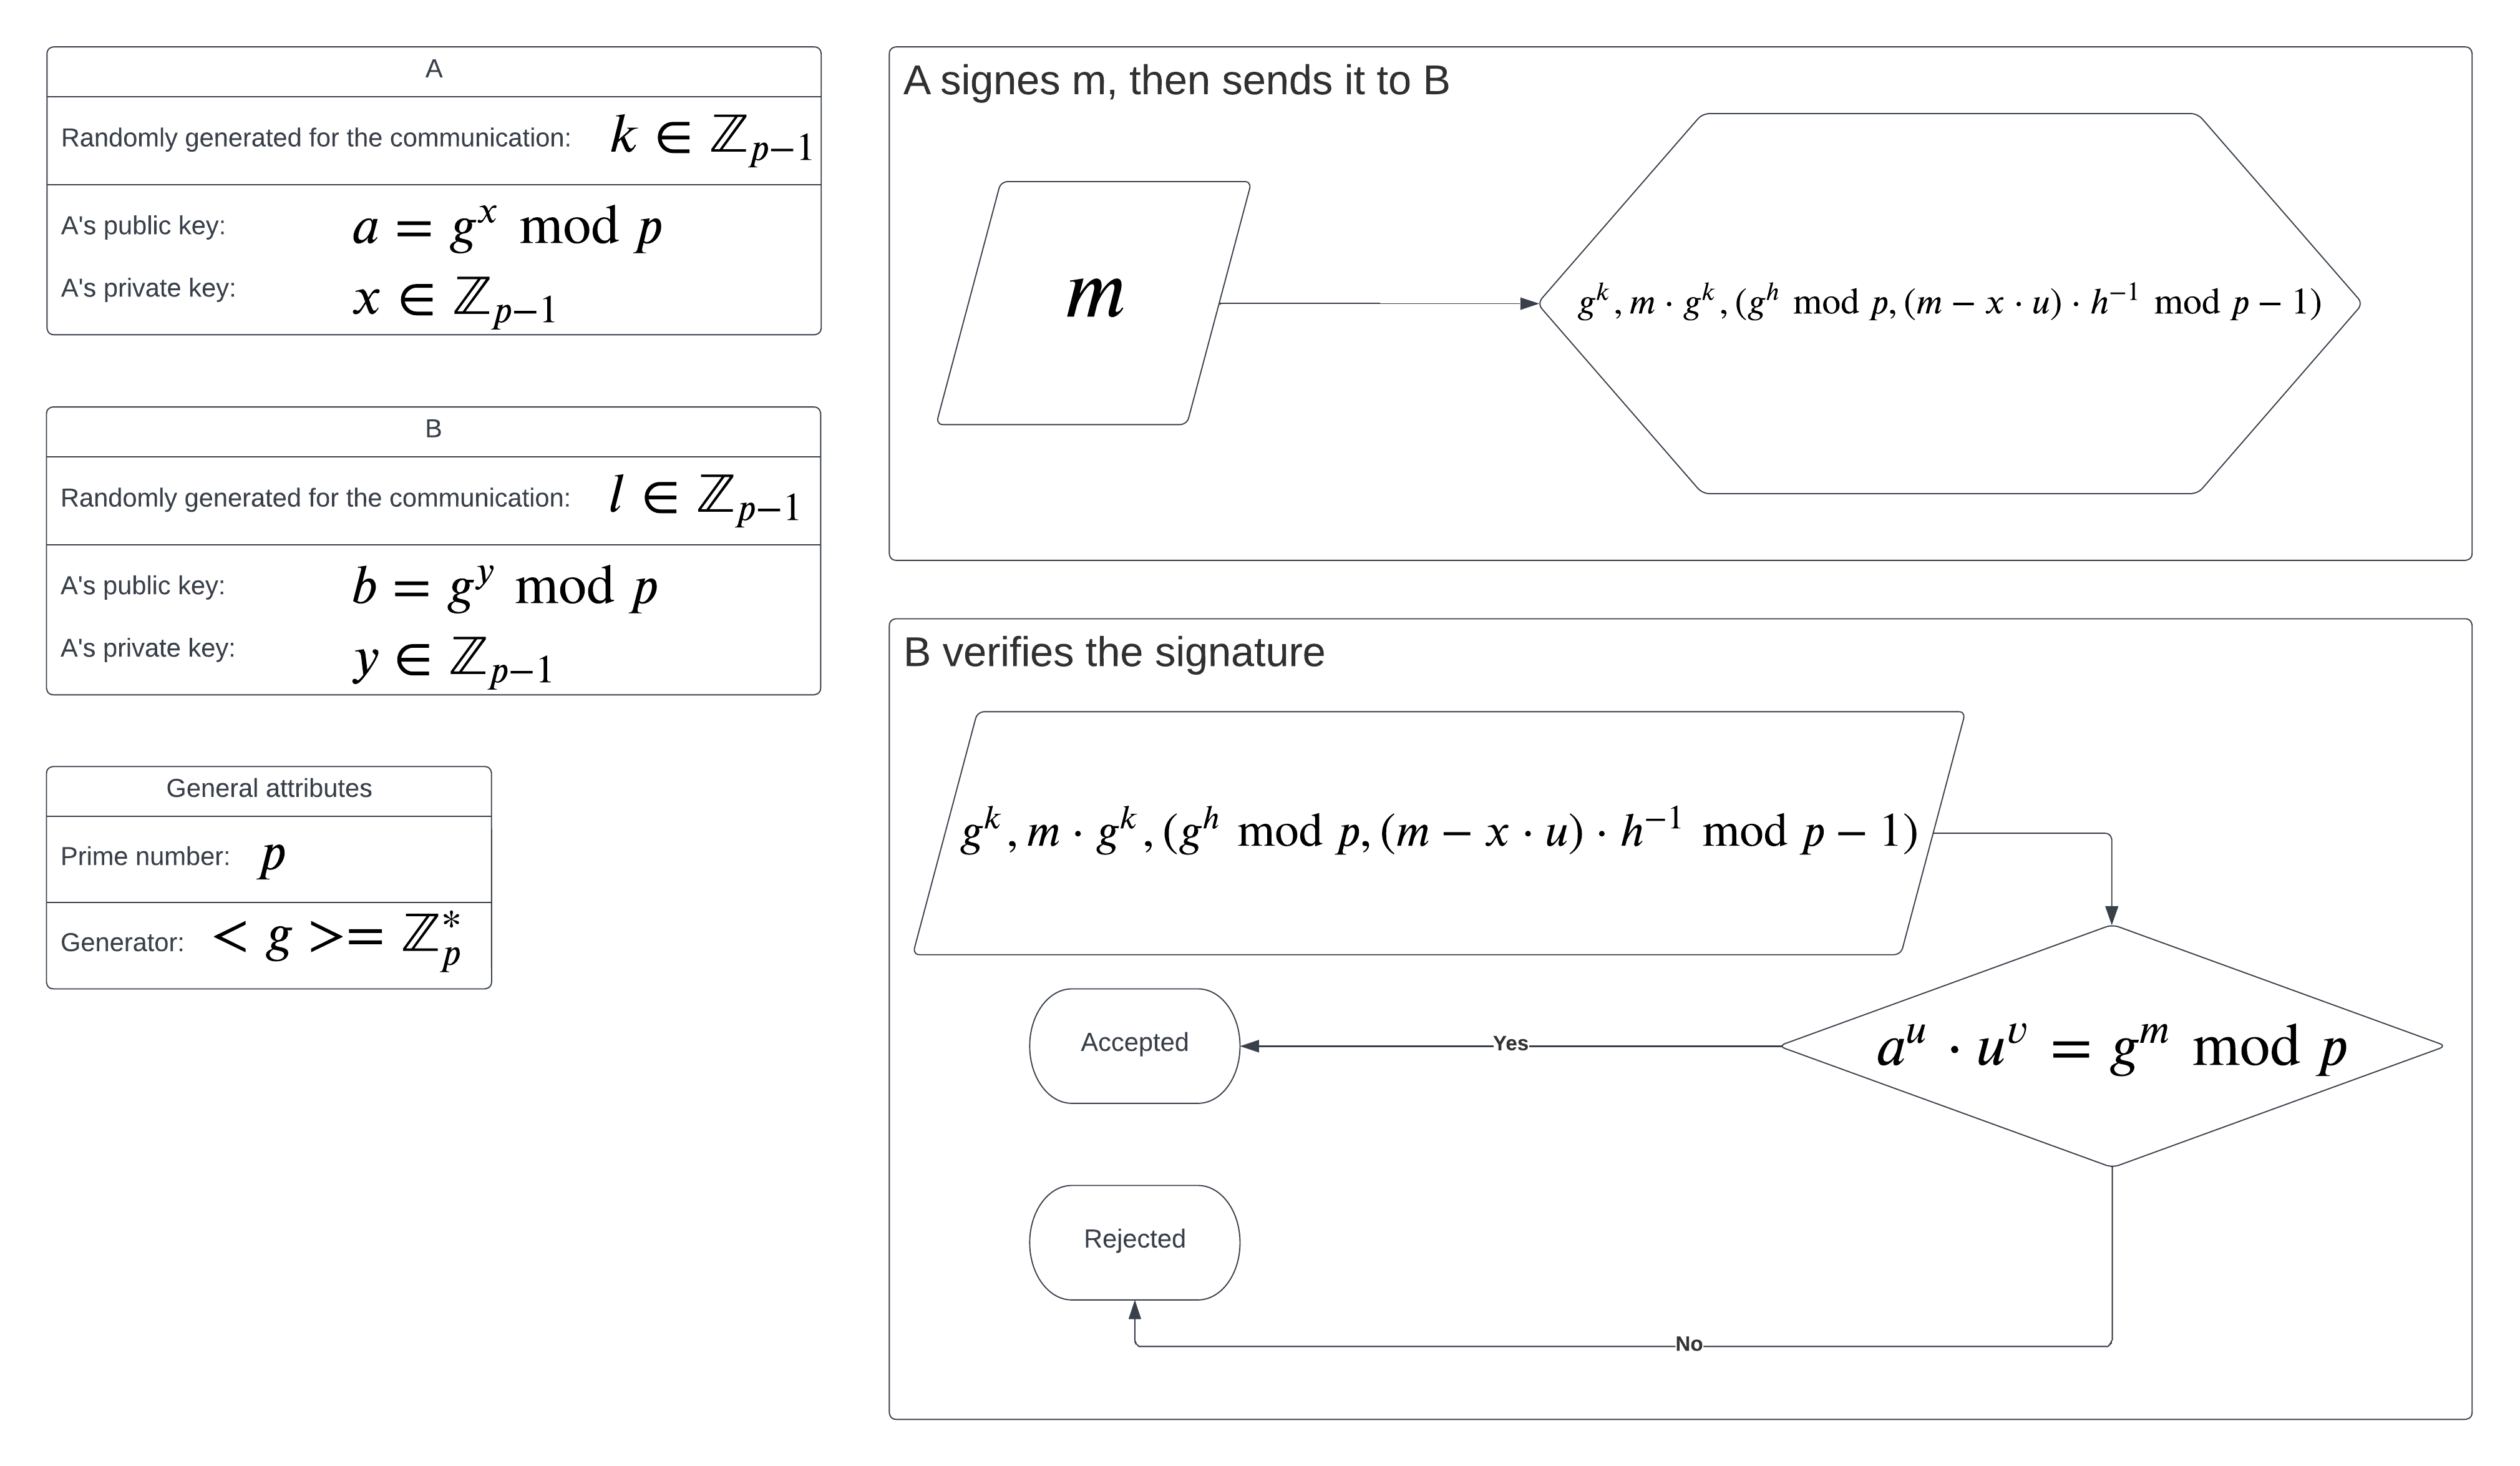
\includegraphics[width=\textwidth]{img/DigSig_ElG.png}
    \caption{Digital signature based on Elgamal cryptosystem.}
\end{figure}
